\textbf{Problem 1: Finite Element Approximation.}

\begin{enumerate}[label=(\alph*),leftmargin=*,itemsep=0mm]
    
    \item Show that $u(\underline{\mu}) \in X\equiv H^1(\Omega)$ satisfies the weak form
    \begin{align}
        a(u(\underline{\mu}),v\mid\underline{\mu}) = l(v),\qquad\forall\>v\in X
    \end{align}
    
    with
    \begin{align}\begin{split}
        a(w,v\mid \underline{\mu})
        &= \sum_{i=0}^4 k^i \int_{\Omega^i} \nabla w\cdot \nabla v \dd{A}
        + \text{Bi} \int_{\Gamma\setminus\Gamma_\text{root}} wv \dd{S} \\
        l(v) &= \int_{\Gamma_\text{root}} v\dd{S}
    \end{split}\end{align}
    
    \begin{proof}
    
    We begin with the Eqn. (1), and multiplying by $v$ we obtain:
    \begin{align*}
        -vk^i\nabla^2u^i = 0
    \end{align*}
    
    Recognising the fact that $\nabla\cdot(v\nabla u) = v\nabla^2u + \nabla v\cdot\nabla u$, we have for the domains $\Omega^i$:
    \begin{align}
        \nabla v \cdot \nabla u^i - \nabla \cdot (v\nabla u^i) &= 0 \nonumber \\
        \therefore \int_{\Omega^i} \nabla v \cdot \nabla u \dd{A}
        &= \int_{\Omega^i} \nabla \cdot (v\nabla u) \dd{A}
    \end{align}
    
    By Gauss' Theorem that states $\int_\Omega \nabla^2 u\dd{A} = \int_\Gamma \nabla u \cdot \hat{n} \dd{S}$, Eq. (7) then becomes, 
    
    \begin{itemize}
        
        \item \textit{Case 1:} Where $i=1, ...,\> 4$:
        \begin{align}
            \int_{\Omega^i} \nabla v \cdot \nabla u \dd{A}
            &= \int_{\Omega^i} \nabla \cdot (v\nabla u) \dd{A} \nonumber
            = \int_{\Gamma^i} \hat{n} \cdot (v\nabla u) \dd{S}
            =  \int_{\Gamma^i} v\nabla u \cdot \hat{n} \dd{S} \nonumber \\
            &= \int_{\Gamma^i_\text{int}} v\nabla u \cdot \hat{n} \dd{S}
            + \int_{\Gamma^i_\text{ext}} v\nabla u \cdot \hat{n} \dd{S}
        \end{align}
        
        We also note that for the domains $\Omega^i$ where $i=1, ...,\> 4$,
        \begin{align}
            \sum_{i=1}^{4} \int_{\Gamma^i_\text{int}} v\nabla u \cdot \hat{n} \dd{S} =
            - \int_{\Gamma^0_\text{int}} v\nabla u \cdot \hat{n} \dd{S}
        \end{align}
        
        And therefore eventually cancels out.  Therefore Eq. (8) functionally simplifies into
        \begin{align}
            \int_{\Omega^i} \nabla v \cdot \nabla u \dd{A}
            &= \int_{\Gamma^i_\text{ext}} v\nabla u \cdot \hat{n} \dd{S}
            = -\frac{\text{Bi}}{k^i} \int_{\Gamma^i_\text{ext}} u^i v \dd{S}
        \end{align}
        
        \item \textit{Case 2:} Where $i=0$:
        \begin{align}
            \int_{\Omega^0} \nabla v \cdot \nabla u \dd{A}
            &= \int_{\Omega^0} \nabla \cdot (v\nabla u) \dd{A} \nonumber
            = \int_{\Gamma^0} \hat{n} \cdot (v\nabla u) \dd{S}
            =  \int_{\Gamma^0} v\nabla u \cdot \hat{n} \dd{S} \nonumber \\
            &= \int_{\Gamma^0_\text{int}} v\nabla u \cdot \hat{n} \dd{S}
            + \int_{\Gamma_\text{root}} v\nabla u \cdot \hat{n} \dd{S}
        \end{align}
        
        From Eq. (9), we see that Eq. (11) functionally simplifies into
        \begin{align}
            \int_{\Omega^0} \nabla v \cdot \nabla u \dd{A}
            &= \int_{\Gamma_\text{root}} v\nabla u \cdot \hat{n} \dd{S}
            = \int_{\Gamma_\text{root}} v \dd{S}
        \end{align}
        
    \end{itemize}
    
    Therefore, summing up Cases 1 and 2, we obtain
    \begin{align*}
        \sum_{i=0}^4 k^i \int_{\Omega^i} \nabla v \cdot \nabla u \dd{A}
        &= - \sum_{i=1}^4 \text{Bi} \int_{\Gamma^i_\text{ext}} u^i v \dd{S}
        + \int_{\Gamma_\text{root}} v \dd{S} \\
        &= - \text{Bi} \int_{\Gamma\setminus\Gamma_\text{root}} u v \dd{S}
        + \int_{\Gamma_\text{root}} v \dd{S}
    \end{align*}
    
    Or, rewritten
    \begin{align}
        \sum_{i=0}^4 k^i \int_{\Omega^i} \nabla v \cdot \nabla u \dd{A}
        + \text{Bi} \int_{\Gamma\setminus\Gamma_\text{root}} u v \dd{S}
        = \int_{\Gamma_\text{root}} v \dd{S}
    \end{align}
    
    Therefore, we see that Eqns. (5) and (6) are satisfied.
    
    \end{proof}
    
    \item Show that $u(\underline{\mu})$ minimizes
    \begin{align}
        J(w) &= \frac{1}{2}\sum_{i=0}^4 k^i \int_{\Omega^i} \nabla w\cdot \nabla w \dd{A}
        + \frac{\text{Bi}}{2} \int_{\Gamma\setminus\Gamma_\text{root}} w^2 \dd{S}
        - \int_{\Gamma_\text{root}} w \dd{S}
    \end{align}
    
    \begin{proof}
    
    Assume that $u$ minimizes $J(w)$ such that
    \begin{gather*}
        u = \arg\min_{w\in X}J(w) = \frac{1}{2}a(w,w) - l(w) \\
        \Updownarrow \\
        a(u,v) = l(v), \qquad \forall\>v\in X
    \end{gather*}
    
    Let us have $w = u + v$, therefore
    \begin{align}
        J(u+v) &= \frac{1}{2} \sum_{i=0}^4 k^i \int_{\Omega^i} \nabla(u+v) \cdot \nabla(u+v) \dd{A} \nonumber \\
        &\quad + \frac{\text{Bi}}{2} \int_{\Gamma\setminus\Gamma_\text{root}} (u+v)^2 \dd{S}
        - \int_{\Gamma_\text{root}} u+v \dd{S} \nonumber \\
        &= \frac{1}{2} \sum_{i=0}^4 k^i
        \int_{\Omega^i} (\nabla u)^2 + 2\nabla u \nabla v + (\nabla v)^2 \dd{A} \nonumber \\
        &\quad + \frac{\text{Bi}}{2} \int_{\Gamma\setminus\Gamma_\text{root}} u^2 + 2uv + v^2 \dd{S}
        - \int_{\Gamma_\text{root}} u+v \dd{S} \nonumber \\
        &= \frac{1}{2} \sum_{i=0}^4 k^i \int_{\Omega^i} (\nabla u)^2 \dd{A}
        + \frac{\text{Bi}}{2} \int_{\Gamma\setminus\Gamma_\text{root}} u^2 \dd{S}
        - \int_{\Gamma_\text{root}} u \dd{S} &&\qquad J(u) \nonumber \\
        &\quad + \sum_{i=0}^4 k^i \int_{\Omega^i} \nabla u\nabla v \dd{A}
        + \text{Bi} \int_{\Gamma\setminus\Gamma_\text{root}} uv \dd{S}
        - \int_{\Gamma_\text{root}} v \dd{S} &&\qquad \delta_vJ(u) \nonumber \\
        &\quad + \frac{1}{2} \sum_{i=0}^4 k^i \int_{\Omega^i} (\nabla v)^2 \dd{S} &&\qquad > 0 \>\text{for}\> v\neq 0
    \end{align}
    
    From Eqns. (10), (12) and (15), we see that $\delta_vJ(u)$ is
    \begin{align*}
        \delta_vJ(u) &= \sum_{i=0}^4 k^i \int_{\Omega^i} \nabla u\nabla v \dd{A}
        + \text{Bi} \int_{\Gamma\setminus\Gamma_\text{root}} uv \dd{S}
        - \int_{\Gamma_\text{root}} v \dd{S} \\
        &= \sum_{i=1}^4 \left( \int_{\Omega^i} \nabla v \cdot \nabla u \dd{A}
        + \text{Bi} \int_{\Gamma^i_\text{ext}} u v \dd{S}\right)
        + \int_{\Omega^0} \nabla v \cdot \nabla u \dd{A}
        + \int_{\Gamma_\text{root}} v \dd{S} \\
        &= 0
    \end{align*}
    
    So Eqn. (15) simplifies to
    \begin{align*}
        J(u+v) &= J(u) + \frac{1}{2} \sum_{i=0}^4 k^i \int_{\Omega^i} (\nabla v)^2 \dd{S} \\
        &\geq J(u)
    \end{align*}
    
    And therefore this means that $u(\underline{\mu})$ is the minimizer of $J(w)$ over all $w \in X$
    
    \end{proof}
    
    \item We consider the linear finite-element space:
    \begin{align*}
        X_h = \{ v\in H^1(\Omega) \mid v|_{T_h} \in \mathbb{P}^1(T_h),\> \forall\> T_h \in \mathcal{T}_h \}
    \end{align*}
    
    In this space we solve for $u(\underline{\mu})$ using the matrix equations:
    \begin{align*}
        \underline{A}_h\underline{u}_h(\underline{\mu}) &= \underline{F}_h \\
        T_{\text{root}.h} &= (\underline{L}_h)^T \underline{u}_h(\underline{\mu})
    \end{align*}
    
    where $\underline{A}_h\in\mathbb{R}^{n\times n}$, $\underline{u}_h\in\mathbb{R}^n$, $\underline{F}_h\in\mathbb{R}^n$ and $\underline{L}_h\in\mathbb{R}^n$, where $n$ is the dimension of the finite element space, which is equal to the number of nodes in $\mathcal{T}_h$.
    
    We first derive the elemental matrices $\underline{A}_h^k\in\mathbb{R}^{3\times 3}$, load vectors $\underline{F}_h^k\in\mathbb{R}^3$ and output vectors $\underline{L}_h^k\in\mathbb{R}^3$ and the describe the procedure for mapping them to $\underline{A}_h$, $\underline{F}_h$ and $\underline{L}_h$.  There are three cases we need to consider:
    
    \begin{itemize}
        
        \item \textit{Case 1:} The Interior Nodes.
        
        The following equation is satisfied:
        \begin{align*}
            \sum_{i=0}^4 k^i \int_{\Omega^i} \frac{\partial{u}}{\partial{x}} \frac{\partial{v}}{\partial{x}}
            + \frac{\partial{u}}{\partial{y}} \frac{\partial{v}}{\partial{y}} \dd{A} = 0
        \end{align*}
        
        Let
        \begin{align*}
            \underline{u}_h &= \sum_{j=1}^n \underline{u}_{h\mid j} \phi_j(x) \\
            v &= \phi_i(x) && \quad \text{for}\> i=1, ...\>, h
        \end{align*}
        
        Then because the points are in the interior, $\underline{A}_h\underline{u}_h = 0$, where $\underline{A}_{h\mid i,j}$ is given by
        \begin{align}
            \underline{A}_{h\mid i,j} &= a(\phi_i,\phi_j)
            = k^i \int_{\Omega^i} \frac{\partial{\phi_i}}{\partial{x}} \frac{\partial{\phi_j}}{\partial{x}}
            + \frac{\partial{\phi_i}}{\partial{y}} \frac{\partial{\phi_j}}{\partial{y}} \dd{A}
        \end{align}
        
        Let us now assume a local triangular element $T_h^k \in T_h$.  Each of these elements have local basis functions $\mathcal{H}_\alpha^k \in \mathbb{P}_1(T_h^k)$, where $\alpha = 1,2,3$, such that
        \begin{align*}
            \mathcal{H}_\alpha^k = c_\alpha + c_{x\mid\alpha}x + c_{y\mid\alpha}y
        \end{align*}
        
        This local triangular element $T_h^k$ has nodes at the points $\underline{x}^k_\beta = (x^k_\beta,y^k_\beta)$, where $\beta = 1,2,3$, which can be mapped to their respective points on the global domain.  From the notes, we can therefore construct the following system of equations:
        \begin{align}
            \begin{pmatrix} 1 & x_1^k & y_1^k \\ 1 & x_2^k & y_2^k \\ 1 & x_3^k & y_3^k \end{pmatrix}
            \begin{pmatrix}
                c_1 & c_2 & c_3 \\ 
                c_{x\mid1} & c_{x\mid2} & c_{x\mid3} \\ 
                c_{y\mid1} & c_{y\mid2} & c_{y\mid3} 
            \end{pmatrix}
            = \begin{pmatrix} 1 & 0 & 0 \\ 0 & 1 & 0 \\ 0 & 0 & 1 \end{pmatrix}
        \end{align}
        
        Therefore, for $\underline{A}_h^k\in\mathbb{R}^{3\times 3}$, the element $\underline{A}_{h\mid\alpha,\beta}^k$ can be calculated by the following (taken from the notes):
        \begin{align}
            \underline{A}_{\alpha,\beta}^k = \text{Area}^k \cdot k_i
            (c_{x\mid\alpha}c_{x\mid\beta} + c_{y\mid\alpha}c_{y\mid\beta}) &&\quad
            1 \leq \alpha,\beta \leq 3
        \end{align}
        
        In this problem, the coordinates are given in the code and therefore can be called.  So we can calculate the area of the triangle from the local coordinates $\underline{x}^k_\beta = (x^k_\beta,y^k_\beta)$ as follows:
        \begin{align}
            \text{Area}^k = \frac{1}{2}(x_1^k(y_2^k-y_3^k) + x_2^k(y_3^k-y_1^k) + x_3^k(y_1^k-y_2^k))
        \end{align}
        
        \item \textit{Case 2:} Along the $\Gamma\setminus\Gamma_\text{root}$ Boundary
        
        The following equation is satisfied
        \begin{align*}
            \sum_{i=0}^4 k^i \int_{\Omega^i} \nabla u \nabla v \dd{A}
            + \text{Bi} \int_{\Gamma\setminus\Gamma_\text{root}} uv \dd{S} = 0
        \end{align*}
        
        Again, let
        \begin{align*}
            \underline{u}_h &= \sum_{j=1}^n \underline{u}_{h\mid j} \phi_j(x) \\
            v &= \phi_i(x) && \quad \text{for}\> i=1, ...\>, h
        \end{align*}
        
        Then knowing once again that $\underline{A}_h\underline{u}_h = 0$, where $\underline{A}_{h\mid i,j}$ is given by
        \begin{align}
            \underline{A}_{h\mid i,j} &= a(\phi_i,\phi_j)
            = k^i \int_{\Omega^i} \frac{\partial{\phi_i}}{\partial{x}} \frac{\partial{\phi_j}}{\partial{x}}
            + \frac{\partial{\phi_i}}{\partial{y}} \frac{\partial{\phi_j}}{\partial{y}} \dd{A}
            + \text{Bi} \int_{\Gamma\setminus\Gamma_\text{root}} \phi_i\phi_j \dd{S}
        \end{align}
        
        The first term is handled in \textit{Case 1}, so now, we are only concerned with calculating the second term to add to $\underline{A}_{h\mid i,j}$.
        
        The $\Gamma\setminus\Gamma_\text{root}$ boundaries will form only one side of a local triangular element $T_h^k \in T_h$ (i.e., only requires two nodes).  Therefore, the problem here is reduced to a 1-D problem, with local basis functions $\mathcal{H}_\alpha^k \in \mathbb{P}_1(T_h^k)$, where $\alpha = 1,2$, such that
        \begin{align*}
            \mathcal{H}_1(\zeta) = \frac{1-\zeta}{2},\quad
            \mathcal{H}_2(\zeta) = \frac{1+\zeta}{2}
        \end{align*}
        
        And in this case, $\underline{A}_h^k\in\mathbb{R}^{2\times2}$, where the terms $\underline{A}_{\alpha,\beta}^k$ are given by
        \begin{align*}
            \underline{A}_{\alpha,\beta}^k &= \text{Bi}
            \int_{\Gamma\setminus\Gamma_\text{root}} \phi_i\phi_j \dd{S} \\
            &= \text{Bi} \cdot \frac{\norm{x_2^k-x_1^k}_{L^2}}{2}
            \int_{\Gamma\setminus\Gamma_\text{root}} \mathcal{H}_\alpha\mathcal{H}_\beta \dd{\zeta}
        \end{align*}
        
        Recognising that
        \begin{align*}
            \int_{-1}^1 H_1H_1 \dd{\zeta} = \int_{-1}^1 H_2H_2 \dd{\zeta} = \frac{2}{3}, \qquad
            \int_{-1}^1 H_1H_2 \dd{\zeta} = \frac{1}{3}
        \end{align*}
        
        We have that $\underline{A}_h^k$ is given by
        \begin{align}
            \underline{A}^k &= \text{Bi} \cdot \frac{\norm{x_2^k-x_1^k}_{L^2}}{6}
            \begin{pmatrix} 2 & 1 \\ 1 & 2 \end{pmatrix}
        \end{align}
        
        \item \textit{Case 3:} Along the $\Gamma_\text{root}$ Boundary
        
        The following equation is satisfied
        \begin{align*}
            \sum_{i=0}^4 k^i \int_{\Omega^i} \nabla u \nabla v \dd{A} = \int_{\Gamma_\text{root}} v \dd{S}
        \end{align*}
        
        Let
        \begin{align*}
            \underline{F}_{h\mid i} &= \int_{\Gamma_\text{root}} \phi_i \dd{S}
        \end{align*}
        
        And since the left-hand side is again handled in \textit{Case 1}, we are now only concerned with calculating the right-hand side to add to $\underline{F}_{h\mid i}$.  And similar to \textit{Case 2}, the $\Gamma_\text{root}$ boundaries will form only one side of a local triangular element $T_h^k \in T_h$ (i.e., only requires two nodes).  Therefore, the problem here is reduced to a 1-D problem, with local basis functions $\mathcal{H}_\alpha^k \in \mathbb{P}_1(T_h^k)$, where $\alpha = 1,2$, such that
        \begin{align}
            \underline{F}_{i}^k &= \int_{\Gamma_\text{root}} \phi_i \dd{S}
            = \frac{\norm{x_2^k-x_1^k}_{L^2}}{2} \int_{-1}^1 \mathcal{H}_i \dd{\zeta} \nonumber \\
            \underline{F}^k &= \frac{\norm{x_2^k-x_1^k}_{L^2}}{2}
            \begin{pmatrix} 1 \\ 1 \end{pmatrix}
        \end{align}
        
    \end{itemize}
    
    \newpage
    
    \item We code up the finite-element solver that takes the configuration $\underline{\mu}$ and triangulation $\mathcal{T}_h$ to calculate $u_h(\underline{\mu})$ and $T_{\text{root}.h}$.  We use the default configuation $\underline{\mu} = \{k_1,k_2,k_3,k_4,\text{Bi}\} = \{0.4,0.6,0.8,1.2,0.1\}$, and plot our solution in Fig. \ref{prj2_qn1_control}a.  Using a trapezoidal summation method, we calculate $T_\text{root}= 1.7342$.

    \begin{figure*}[h!]
    \centering
    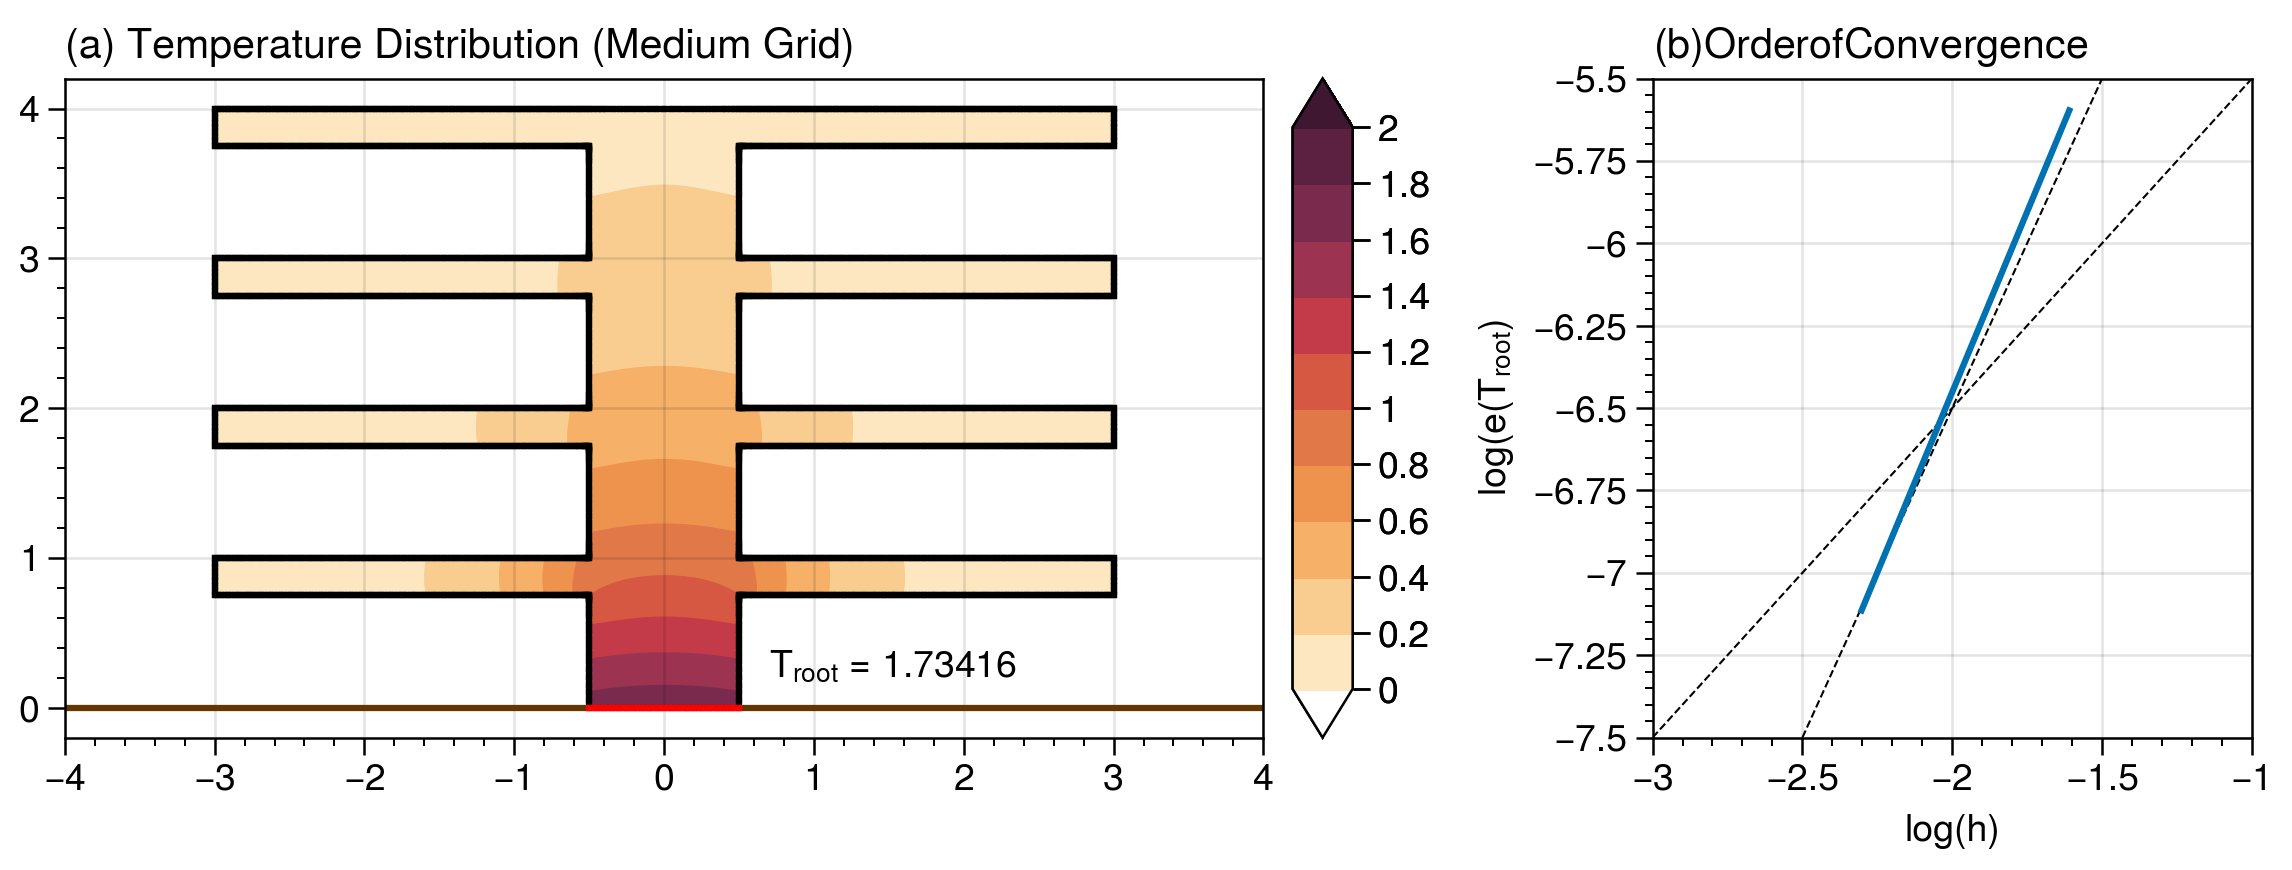
\includegraphics[width=\textwidth]{figures/prj2_qn1_control.png}\\
    \caption{}
    \label{prj2_qn1_control}
    \end{figure*}
    
    \item We wish to show that
    \begin{align}
        T_\text{root}(\underline{\mu}) - T_{\text{root},h}(\underline{\mu})
        = a(e(\underline{\mu}), e(\underline{\mu}))
    \end{align}
    
    where
    \begin{align*}
        e(\underline{\mu}) &= u(\underline{\mu}) - u_h(\underline{\mu}) \\
        T_\text{root}(\underline{\mu}) &= \int_{\Gamma_\text{root}} u \dd{S} \\
        T_{\text{root},h}(\underline{\mu}) &= L_h^T u_h(\underline{\mu})
    \end{align*}
    
    We are given that $l(v) = l^0(v)$
    \begin{align*}
        \therefore T_\text{root}(\underline{\mu}) - T_{\text{root},h}(\underline{\mu})
        &= l^0(u(\underline{\mu})) - l^0(u_h(\underline{\mu})) \\
        &= l(u(\underline{\mu})-u_h(\underline{\mu}))
    \end{align*}
    
    The weak form gives us
    \begin{align*}
        a(u,v) &= l(v), \quad \forall\> v \in X \\
        a(u_h,v') &= l(v'), \quad \forall\> v' \in X_h
    \end{align*}
    
    Let $v = u$ and $v' = u_h$, such that the equations are transformed into
    \begin{gather*}
        a(u,u) = l(u), \quad a(u_h,u_h) = l(u_h)
    \end{gather*}
    
    Using bilinearity and linearity, we obtain
    \begin{align*}
        a(u-u_h,u-u_h) &= l(u-u_h) = T_\text{root}(\underline{\mu}) - T_{\text{root},h}(\underline{\mu}) \\
        \therefore T_\text{root}(\underline{\mu}) - T_{\text{root},h}(\underline{\mu})
        &= a(u-u_h,u-u_h) = a(e(\underline{\mu}), e(\underline{\mu}))
    \end{align*}
    
    Next, we wish to find the convergence of the solution.  Using the coarse, medium and fine grids respectively, we find $T_{\text{root},h} = 1.731266$, 1.734163 and 1.734976.
    
    We use the equation given, that
    \begin{align*}
        T_{\text{root},\text{fine}} - T_{\text{root},\text{medium}} &= C (2h_\text{fine})^b \\
        T_{\text{root},\text{fine}} - T_{\text{root},\text{coarse}} &= C (4h_\text{fine})^b \\
        \therefore \log(\frac{T_{\text{root},\text{fine}} - T_{\text{root},\text{medium}}}{T_{\text{root},\text{fine}} - T_{\text{root},\text{coarse}}}) &= b\log(\frac{1}{2}) \\
        \therefore b &= 2.189
    \end{align*}
    
    And therefore we see that the convergence is 2nd order, as shown in Fig. \ref{prj2_qn1_control}b.
    
\end{enumerate}